%-----------------------------------------------------------------------
\section{Tactical Data Mining}
%-----------------------------------------------------------------------

We convert the structured stroke table into five complementary tactical views.
Each view answers a different question: what strokes are used, how strokes
follow one another, which multi-stroke phrases recur, how movement relates to
stroke choice, and whether high-level profiles cluster into interpretable
groups.

A central methodological commitment of this work is that we validate the
\emph{mining}, not only the perception. The same 3{,}178 evaluated events carry
both predicted and ground-truth stroke labels, so every analysis can be run
twice---once on the predicted stream and once on the matched truth---and the
predicted-vs-true gap measured directly. Table~\ref{tab:mining_eval}
consolidates this evaluation: for each task we list its input, algorithm,
metric, a baseline, and the measured conclusion. The remainder of this section
develops each view and its validation in turn.

\begin{table*}[t]
  \caption{\textbf{Data Mining Evaluation.} Each tactical-mining task is run on
  the predicted stream and on the matched ground-truth stream over the same
  3{,}178 evaluated strokes (videos~41--44). The gap quantifies how much
  tactical signal survives end-to-end prediction. Lower is better for KL,
  $\chi^2$, total variation (TV), and transition error; higher is better for
  overlap, Spearman~$\rho$, and ARI.}
  \label{tab:mining_eval}
  \centering
  \footnotesize
  \setlength{\tabcolsep}{4pt}
  \begin{tabular}{p{1.7cm} p{2.5cm} p{2.6cm} p{2.7cm} p{2.5cm} p{3.4cm}}
    \toprule
    Task & Input & Algorithm & Metric (pred vs.\ true) & Baseline & Measured result \& conclusion \\
    \midrule
    Stroke composition
      & 3{,}178 predicted labels
      & Stroke-frequency aggregation
      & KL, $\chi^2$, TV vs.\ true distribution
      & Uniform dist.\ (KL $0.18$)
      & KL $0.04$, $\chi^2\,0.02$, TV $0.10$; composition $4\times$ closer to truth than uniform \\[2pt]

    Markov transitions
      & 343 rally label sequences
      & First-order row-normalized matrix
      & Frobenius $\lVert T-\hat{T}\rVert_F$, mean row KL
      & Random $2.77$, unigram $2.61$, earlier $3.77$
      & $1.23$ / $0.51$; beats memoryless \& random, recovers attack--defence grammar \\[2pt]

    Frequent motifs
      & Rally token sequences
      & Contiguous $n$-gram rally support ($n{=}2$--$4$)
      & Top-10 Jaccard, overlap@10, Spearman $\rho$
      & Random top-10 overlap $\approx 0$
      & $n{=}3$: $\rho\,0.66$, overlap@10 $0.70$; phrase ranks preserved, decay at $n{=}4$ \\[2pt]

    Movement profiling
      & 2{,}300 player-centric events
      & 12-dim profiles + Pearson $r$
      & Pearson $r$, $95\%$ CI, $p$, BH-FDR ($n{=}16$)
      & $r=0$ (no association)
      & coverage$\to$netward $r{=}{+}0.73$ ($p{=}0.001$, BH-sig); direct smash links $r{=}{+}0.30/{-}0.34$ suggestive only ($p{>}0.2$) \\[2pt]

    Strategy clustering
      & 16 player-set profiles
      & KMeans ($k{=}3$) + silhouette/bootstrap
      & Pred-vs-true ARI, feature fidelity
      & Random labels ARI $\approx 0.00$
      & ARI $0.17$, feature $\bar{r}\,0.79$; profiles faithful, labels descriptive \\
    \bottomrule
  \end{tabular}
\end{table*}

\subsection{Stroke Composition}

Stroke-distribution analysis aggregates top-1 predicted labels across all events
to summarise match composition. The clean predicted stream contains 3{,}178
strokes across 343 rallies with a mean rally length of 9.27 strokes, close to
the annotation-derived mean of 9.91. In the predicted stream, smash ($13.1\%$),
lob ($12.4\%$), and clear ($11.7\%$) form a tight leading band, immediately
followed by drop, return net, and push ($11.3\%$ down to $9.8\%$); net shot and
drive are mid-frequency, while cross-court net shot, the services, and rush
($2.2\%$) are progressively rarer. This near-even split between an attacking
stroke (smash) and rally-sustaining strokes (lob, clear, drop) matches
established singles rally structure, where neutral and defensive strokes
collectively outnumber outright attacks.
Figure~\ref{fig:stroke_distribution} visualizes this predicted stroke
composition.

\paragraph{Validation against ground truth.}
Comparing the predicted stroke-type distribution with the true distribution over
the same events, the Kullback--Leibler divergence is only
$\mathrm{KL}(P_{\text{true}}\Vert P_{\text{pred}})=0.042$, with a symmetric
$\chi^2$ distance of $0.020$ and a total-variation distance of $0.102$. As a
reference, the true distribution sits $\mathrm{KL}=0.178$ from a uniform
distribution, so the predicted composition is roughly $4\times$ closer to truth
than an uninformed baseline (Figure~\ref{fig:mining_validation}a). The one
systematic shift is at the \emph{head} of the ranking: the true stream is led by
lob and net shot ($15.6\%$ and $15.5\%$), but the classifier under-recalls net
shot ($485\to252$ events) and, less severely, lob ($488\to368$) while recovering
smash almost exactly ($387\to387$), which is what promotes smash to the nominal
top of the predicted ranking. Because the displaced mass redistributes across the
adjacent mid-frequency strokes rather than collapsing onto a few labels, the
global divergence stays small ($\mathrm{KL}=0.04$) even as the single most
frequent stroke changes. The recovered match composition is therefore
quantitatively faithful in aggregate, with a known under-recall of net shot as
its main local distortion.

\begin{figure}[t]
  \centering
  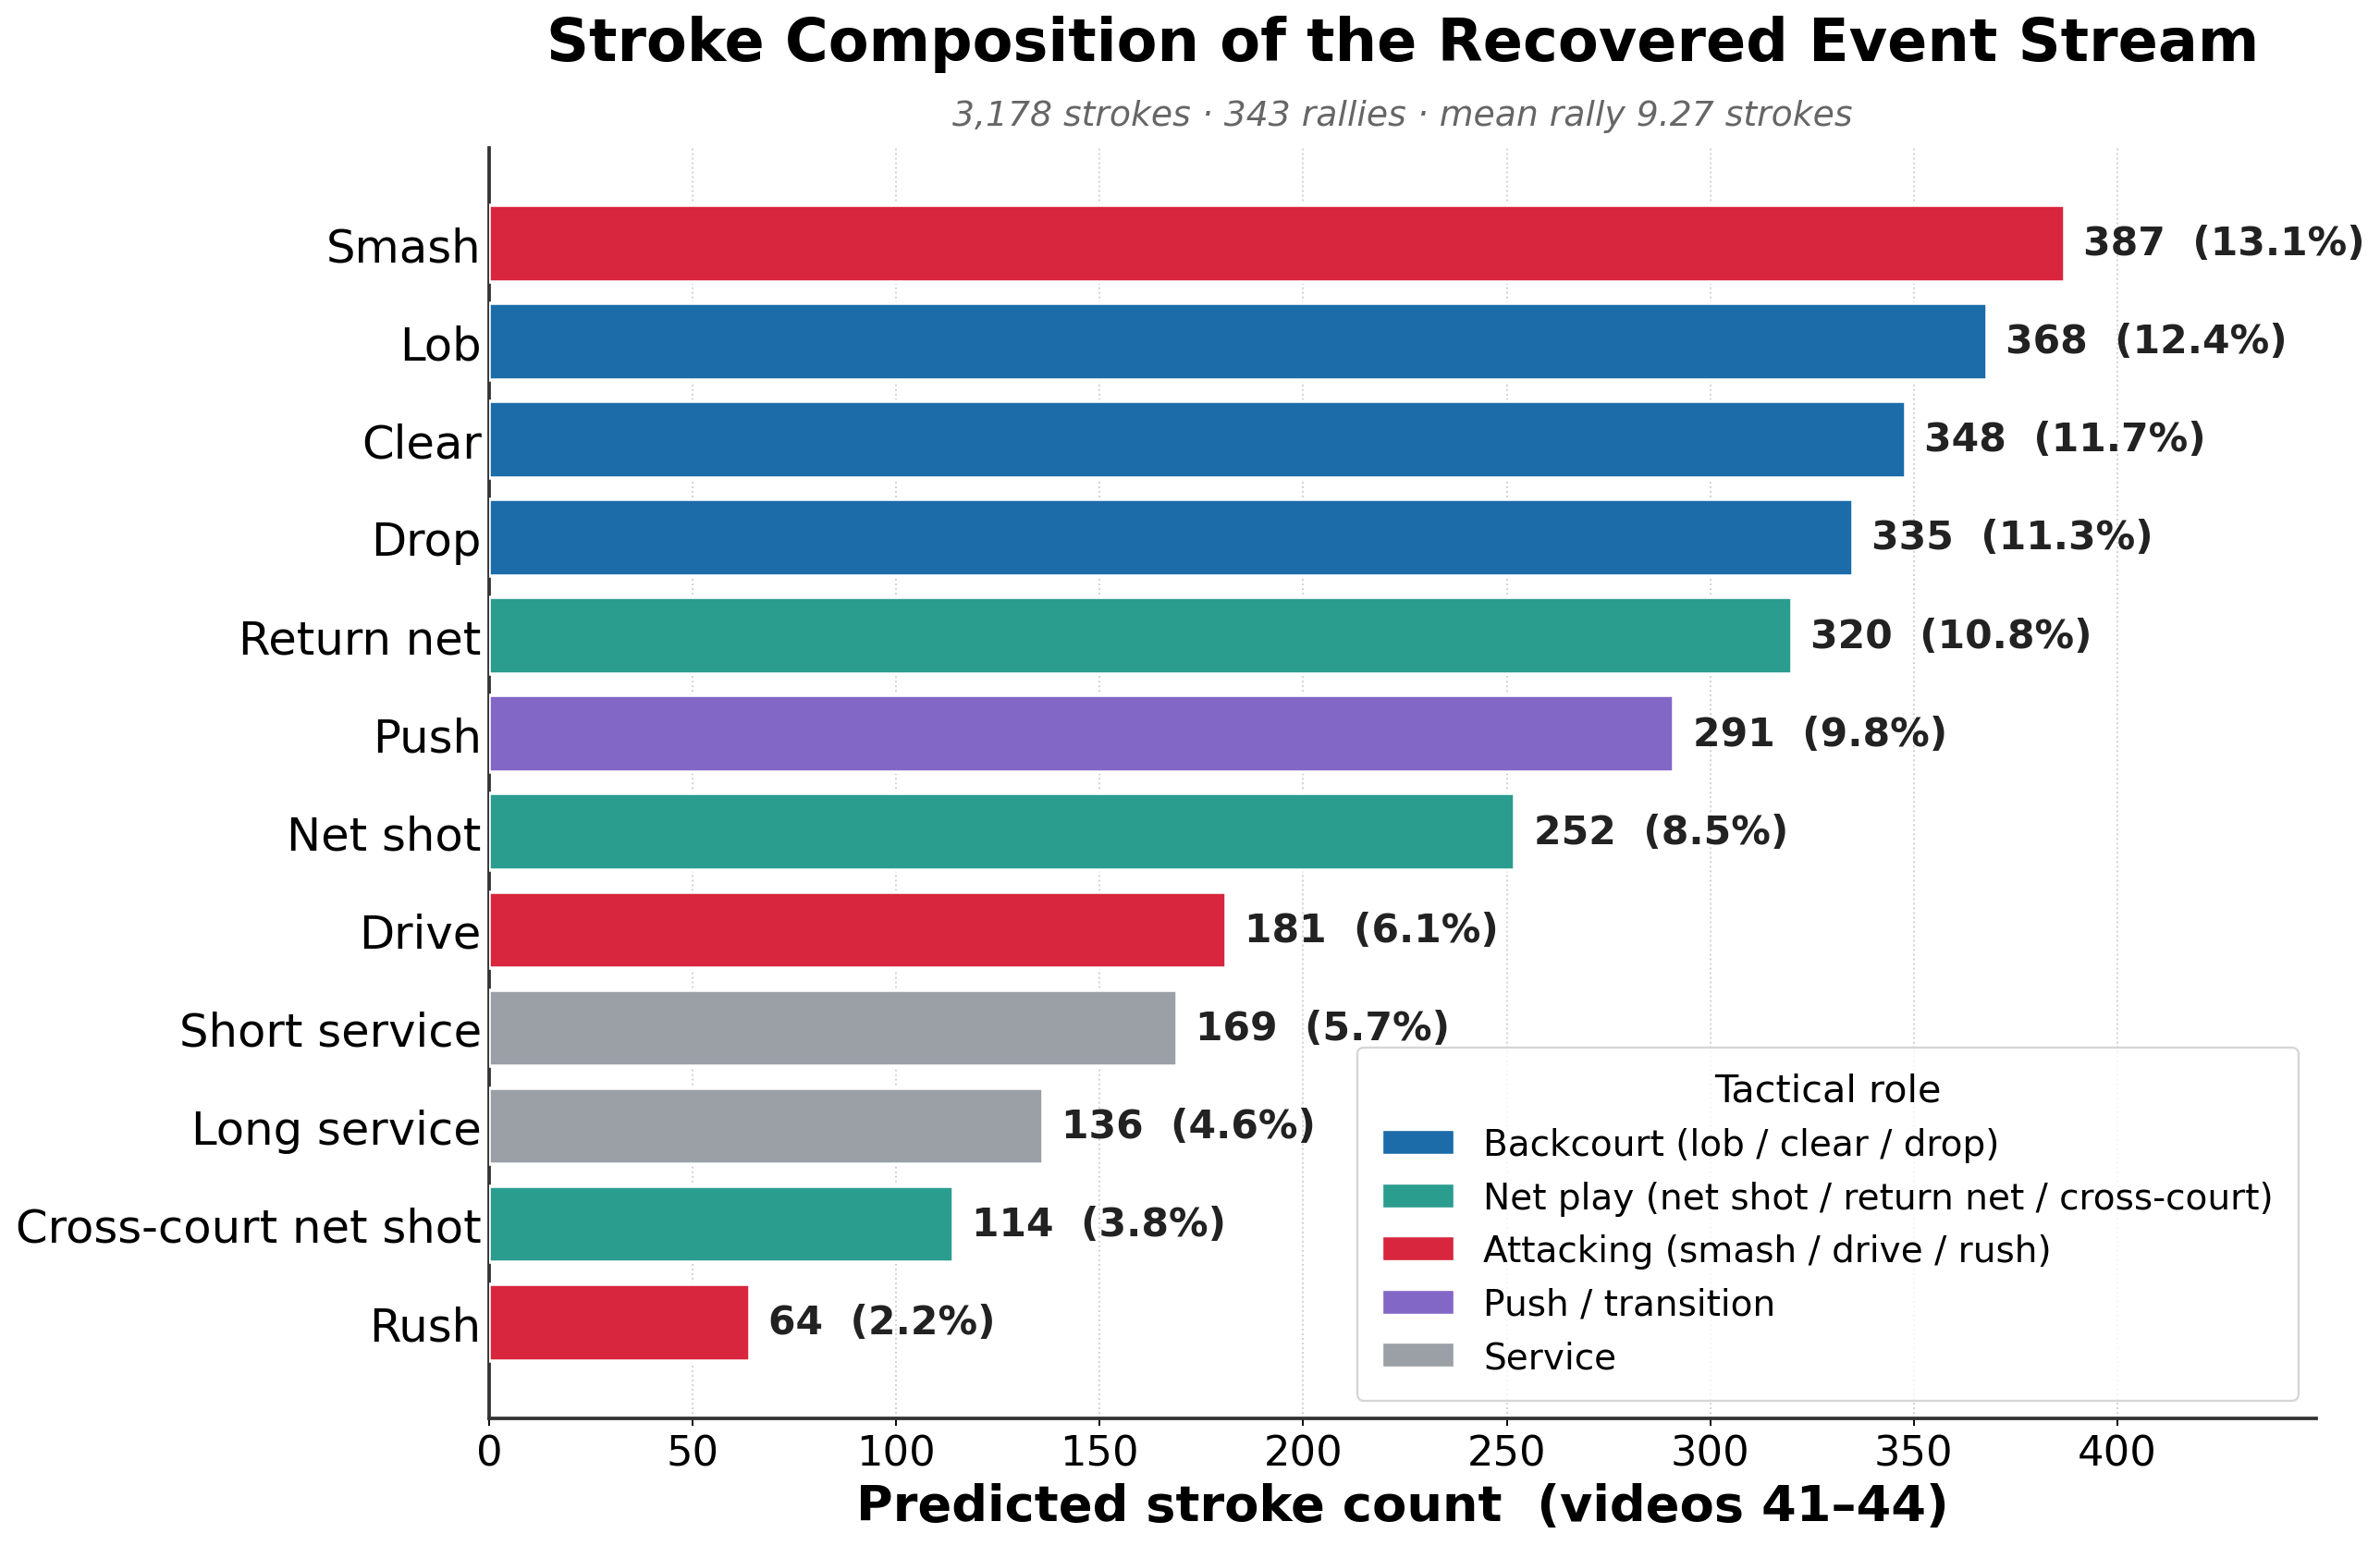
\includegraphics[width=\linewidth]{images/stroke_distribution.png}
  \caption{\textbf{Stroke composition.} Distribution of predicted stroke types (side-agnostic) across the unseen evaluation set. Smash, lob, and clear form a tight leading band, followed by drop, return net, and push, reflecting a near-even mix of attacking and rally-sustaining strokes.}
  \label{fig:stroke_distribution}
\end{figure}

\subsection{Markov Transitions}

Markov modeling converts each rally into stroke-to-stroke transitions and builds
a transition matrix whose rows index the current stroke and columns index the
next. Let $C_{ij}$ denote the number of times stroke $i$ is immediately
followed by stroke $j$ in the data; the corresponding row-normalised
transition probability is
\[
T_{ij} = \frac{C_{ij}}{\sum_k C_{ik}},
\]
which defines a first-order Markov chain over the stroke vocabulary.
This matrix answers: given a stroke, what reply tends to follow next?
To quantify how well the predicted matrix \(\hat{T}\) matches the ground
truth \(T\), we report the Frobenius norm
\(\|T - \hat{T}\|_F = \sqrt{\sum_{ij}(T_{ij} - \hat{T}_{ij})^2}\)
and the per-row Kullback--Leibler divergence
\(\mathrm{KL}(T_i \Vert \hat{T}_i) = \sum_j T_{ij} \log\frac{T_{ij}}{\hat{T}_{ij}}\).
Reducing the \texttt{none} rate from 56.43\% to 6.70\% cuts the Frobenius error
from 3.77 to 1.23 and the mean row KL from 11.55 to 0.51---roughly a $67\%$ and
$96\%$ reduction---when both pipelines are scored against the \emph{same}
3{,}178-event ground-truth reference (the earlier-pipeline caveat and its
own-reference score are detailed in Table~\ref{tab:transition_baselines}).

\paragraph{Transition baselines.}
A raw error of $1.23$ is only meaningful against a yardstick, so
Table~\ref{tab:transition_baselines} places the predicted matrix between two
naive references and an ablation baseline, all scored against the same
ground-truth transitions. The \emph{earlier pipeline} in that table is a prior
version of \method{} that used a weaker pose model and no BST fine-tuning: it
predicted the \texttt{none} class for 56.43\% of all stroke windows, meaning
more than half the rally sequence was discarded before any mining could begin.
We include it to quantify the cost of broken sequence coherence---not as a
comparison with an external system, but as an internal ablation showing how much
the \texttt{none}-reduction step is worth. A \emph{uniform-random} row-normalized matrix scores
$2.77$, and a \emph{unigram} (memoryless) model---every row set equal to the
marginal next-stroke distribution, i.e.\ ignoring the current stroke---scores
$2.61$. The current pipeline ($1.23$) more than halves both, which is the key
evidence that the recovered transitions encode genuine first-order structure
rather than merely reproducing overall stroke frequencies. By contrast, the
earlier \texttt{none}-flooded pipeline ($3.77$ on the same reference) is
\emph{worse than even the random baseline}: collapsing half of all rows onto the
\texttt{none} column
pushes the matrix further from ground truth than chance, a concrete illustration
of how broken sequence coherence destroys transition structure.

\begin{table}[t]
  \caption{Transition-recovery baselines. Frobenius and mean row-KL distance to
  the matched ground-truth transition matrix on the 3{,}178-event set (25
  side-aware states). All five rows share this single reference; the earlier
  pipeline's predicted matrix is estimated from its own 2{,}986-event run but
  compared against the identical reference (against its own matched truth it
  scores a near-identical 3.65 / 11.72). Lower is better.}
  \label{tab:transition_baselines}
  \centering
  \small
  \begin{tabular}{lrr}
    \toprule
    Transition model & Frobenius\,$\downarrow$ & Mean row KL\,$\downarrow$ \\
    \midrule
    Uniform-random rows              & 2.77 & 2.23 \\
    Unigram (memoryless)             & 2.61 & 1.58 \\
    Earlier pipeline (\texttt{none} 56.4\%) & 3.77 & 11.55 \\
    Current pipeline (\texttt{none} 6.7\%)  & \textbf{1.23} & \textbf{0.51} \\
    Ground truth (reference)         & 0.00 & 0.00 \\
    \bottomrule
  \end{tabular}
\end{table}

\paragraph{Attack--defence grammar.}
All transition probabilities below are computed from the 3{,}178 predicted
strokes across four elite matches: Ng Ka Long Angus vs.\ Kidambi Srikanth
(QF), Sindhu vs.\ Chochuwong (QF), Marin vs.\ Chochuwong (SF), and
Antonsen vs.\ Axelsen (Finals) --- all from the HSBC BWF World Tour Finals
2020. Side labels (Top/Bottom) are camera-relative; figures are reported
after pooling both sides.

\textbf{Net shot is the primary setup stroke.}
Net shots force a lob reply 52.0\% of the time and a push 20.9\%,
making them the most reliable stroke for creating an attacking opportunity
rather than winning the point directly. The remaining 20.3\% sees the
opponent answer with another net shot, initiating a net-zone exchange.

\textbf{Lob and clear both invite attacking replies, through different paths.}
After a lob, the opponent smashes 41.6\% of the time and drops 29.1\%,
with only 24.2\% answered by a clearing reply. After a clear, the split is
almost three-way: smash 35.3\%, clear-to-clear 30.6\%, and drop 30.4\%.
The clear-to-clear continuation is the predicted ``waiting game'': neither
player commits to an attack until a sufficiently weak ball arrives.
This three-way branching after a clear is a key distinction from the lob,
where the attacking smash is the dominant choice.

\textbf{Smash almost never ends the rally.}
Across the four matches, 61.9\% of smashes draw a return net (defensive
block), 11.8\% a drive, and 11.7\% a cross-court net shot. Fewer than 3\%
of smashes are followed by a lob or net shot---meaning the rally almost
always continues. The smash accumulates pressure rather than finishing
points.

\textbf{Drop opens net play.}
A drop is answered with a net shot 21.4\% of the time, a push 16.7\%, or
a cross-court net shot 11.7\%, placing roughly half of drop replies into
the net zone. This positions the dropping player to threaten with a
subsequent net attack or rush.

\textbf{Defensive return restores neutral.}
After a return net, the most common reply is a push (31.5\%) or lob (23.4\%),
resetting the rally to a neutral net-zone or backcourt exchange rather than
immediately launching another attack.

Together these five patterns form a repeating rally cycle
(Figure~\ref{fig:transition_heatmap}):
net shot $\rightarrow$ lob $\rightarrow$ smash $\rightarrow$ return net
$\rightarrow$ push/lob $\rightarrow$ net shot, punctuated by the
backcourt ``waiting'' phase (clear $\rightarrow$ clear $\rightarrow$ smash)
whenever both players retreat to consolidate position.

\begin{figure}[t]
  \centering
  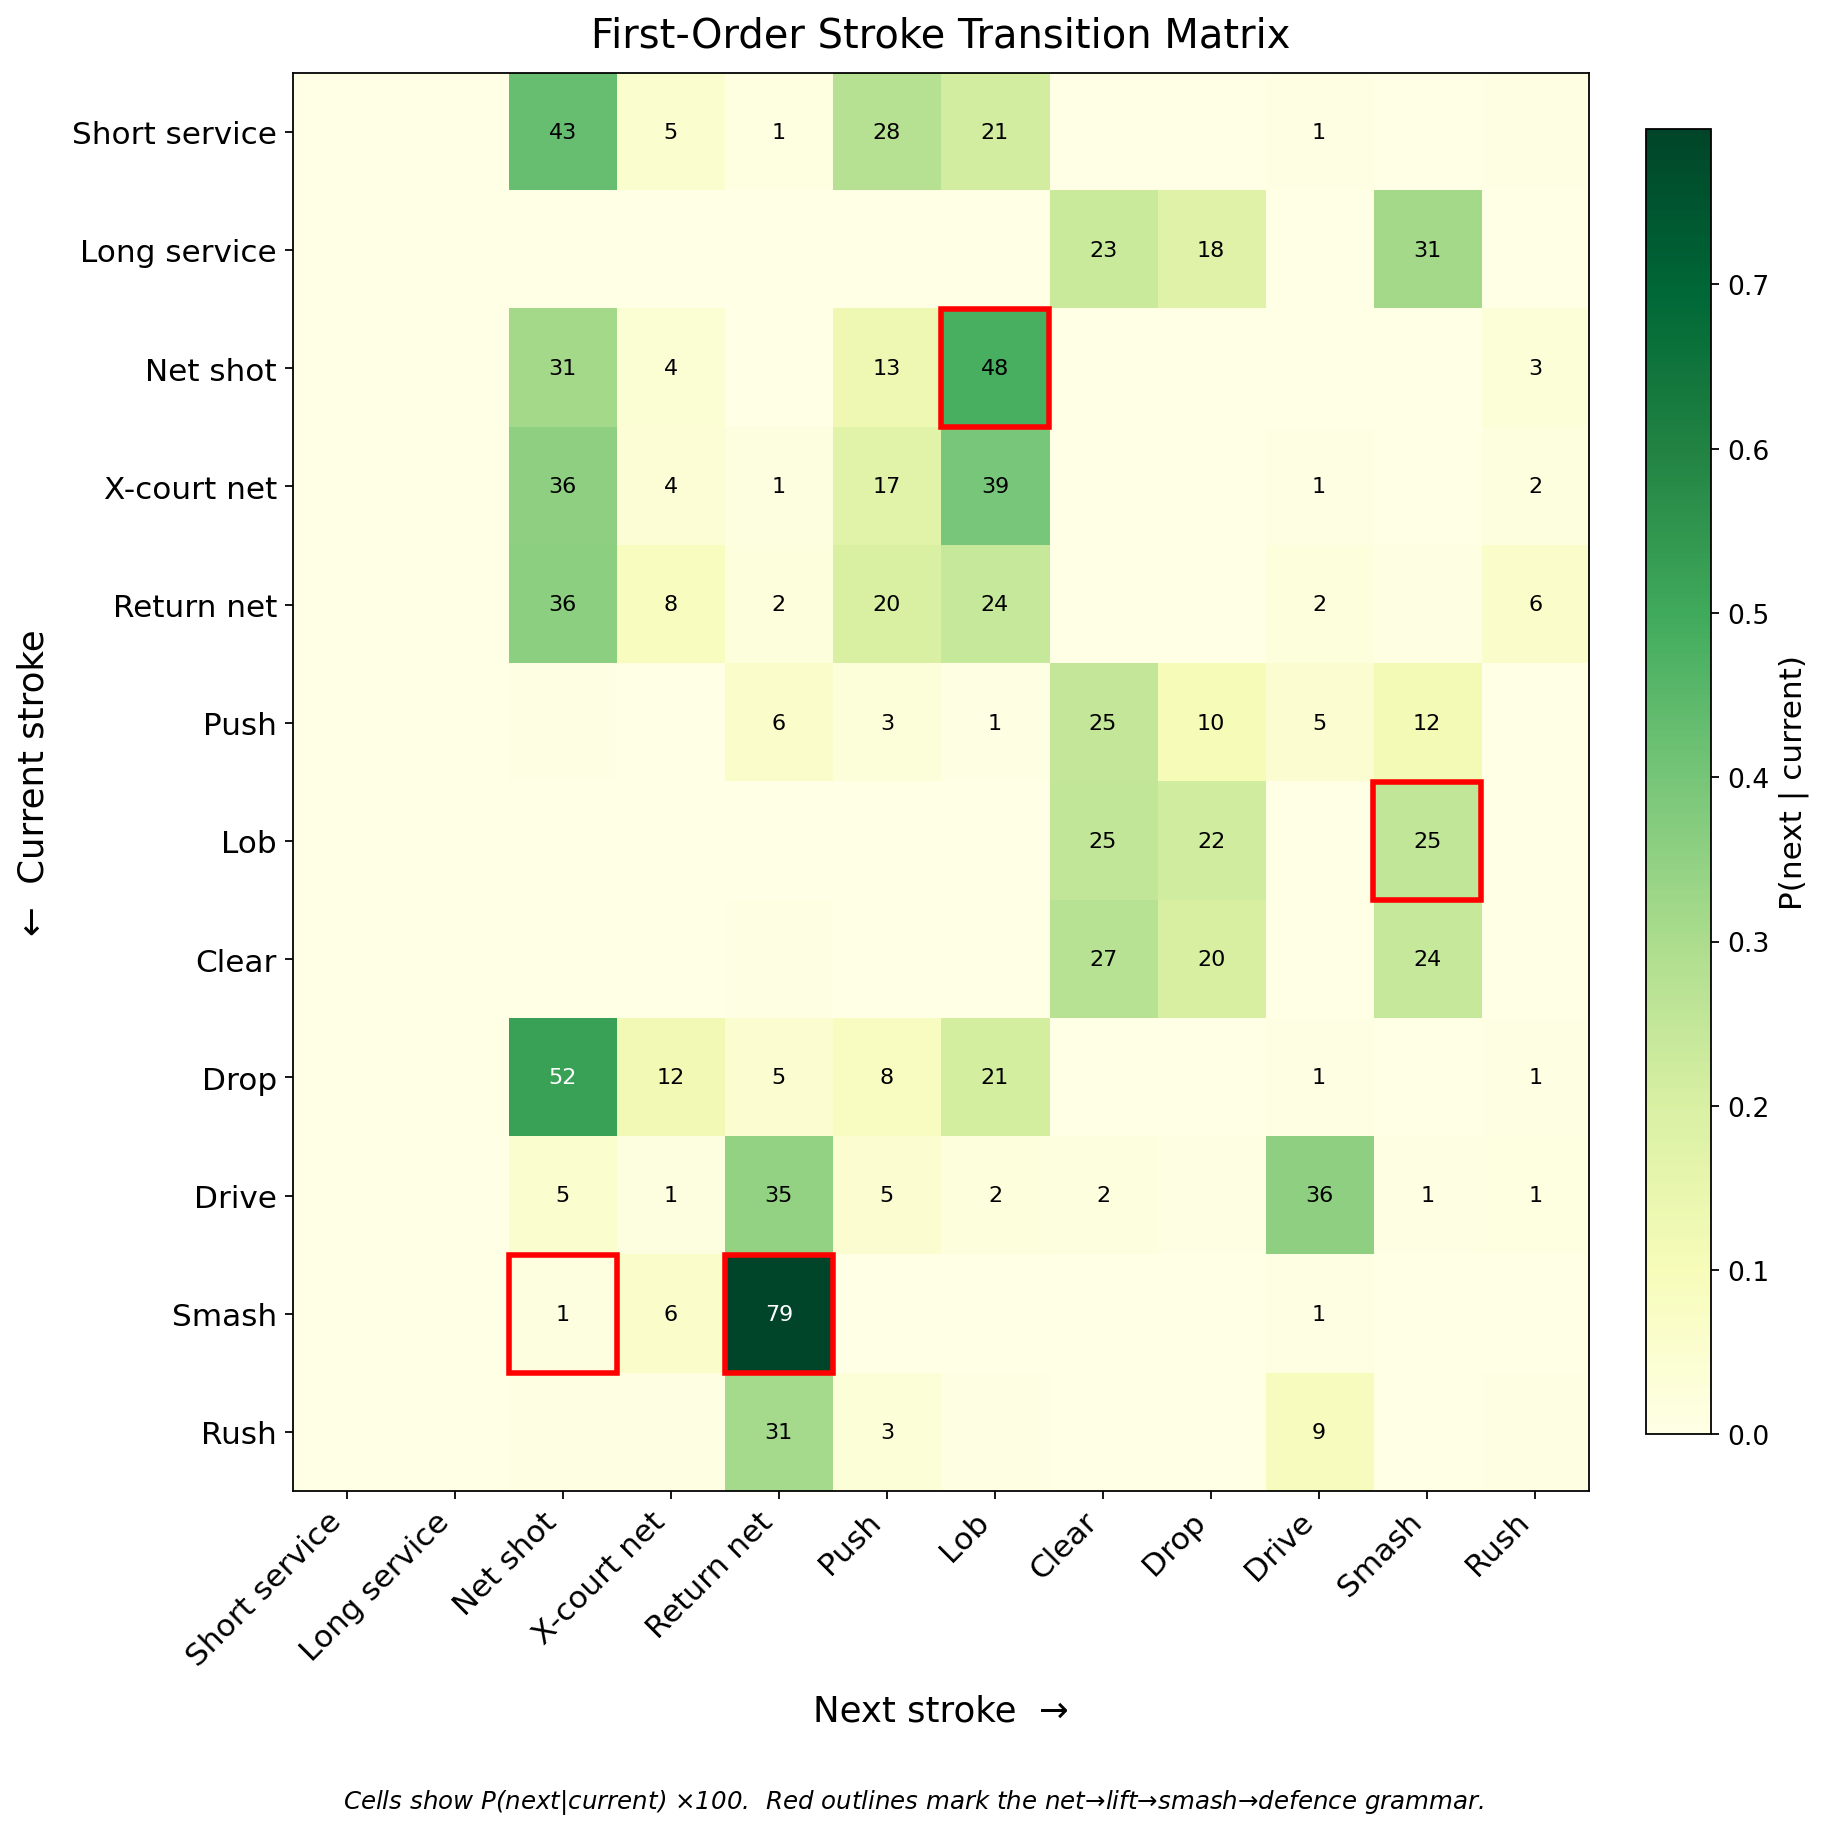
\includegraphics[width=\linewidth]{images/transition_heatmap.png}
  \caption{\textbf{Transition matrix.} First-order stroke-transition matrix
  from the predicted event stream across videos~41--44 (side-agnostic,
  \texttt{none} excluded). Each cell reports
  $P(\text{next}\mid\text{current})\times100$; rows index the current stroke
  and columns the next. Red outlines mark the recovered attack--defence
  grammar: net~$\rightarrow$~lob, lob/clear~$\rightarrow$~smash,
  smash~$\rightarrow$~return net, and clear~$\rightarrow$~clear (backcourt
  waiting exchange).}
  \label{fig:transition_heatmap}
\end{figure}

\subsection{Frequent Motif Mining}

Motif mining extends Markov analysis from single transitions to repeated
multi-stroke phrases. Contiguous $n$-grams are ranked by \emph{rally support},
defined for a motif $m$ as
\[
\mathrm{support}(m) = \frac{\#\{\text{rallies containing } m\}}{\#\{\text{total rallies}\}},
\]
the fraction of rallies that contain at least one instance of $m$.  In the
ground truth, the dominant motif is net~$\rightarrow$~lob~$\rightarrow$~smash~$\rightarrow$~defensive
reply, which appears in about 11\% of rallies. The predicted stream recovers
this structure in side-aware form: Top net~$\rightarrow$~Bottom lob~$\rightarrow$~Top
smash~$\rightarrow$~Bottom return net appears in 4.7\% of rallies, and shorter
sub-sequences are common. Motif mining thus translates the transition matrix
into an interpretable tactical phrase: net pressure induces a lift, the lift
creates attacking opportunity, and the attack draws a defensive reply.
Figure~\ref{fig:motif_support} reports the rally support of the most frequent
motifs and highlights which repeated phrases occur most reliably.

\paragraph{Validation against ground truth.}
Mining the same rallies from the matched true labels, the dominant four-stroke
phrase net~$\rightarrow$~lob~$\rightarrow$~smash~$\rightarrow$~return net occurs
in $12.2\%$ of true rallies and is recovered as the single most frequent
predicted motif ($7.1\%$ side-agnostic; $4.7\%$ in strict side-aware form). To
quantify agreement beyond the top phrase, we compare predicted and true motif
\emph{supports} across all motifs above $2\%$ rally support. The rankings agree
well at tactical-phrase scale---Spearman $\rho=0.85$ for pairs ($n{=}2$) and
$\rho=0.66$ for triples ($n{=}3$), with top-10 overlap@10 of $0.60$ and $0.70$
(Jaccard $0.43$ and $0.54$)---but degrade for four-grams ($\rho=0.32$,
overlap@10 $0.40$) as longer phrases compound per-stroke errors
(Figure~\ref{fig:mining_validation}b). The
mined tactical grammar is thus reliable at the two- and three-stroke scale that
carries most coaching value, with longer phrases interpreted more cautiously.

\begin{figure}[t]
  \centering
  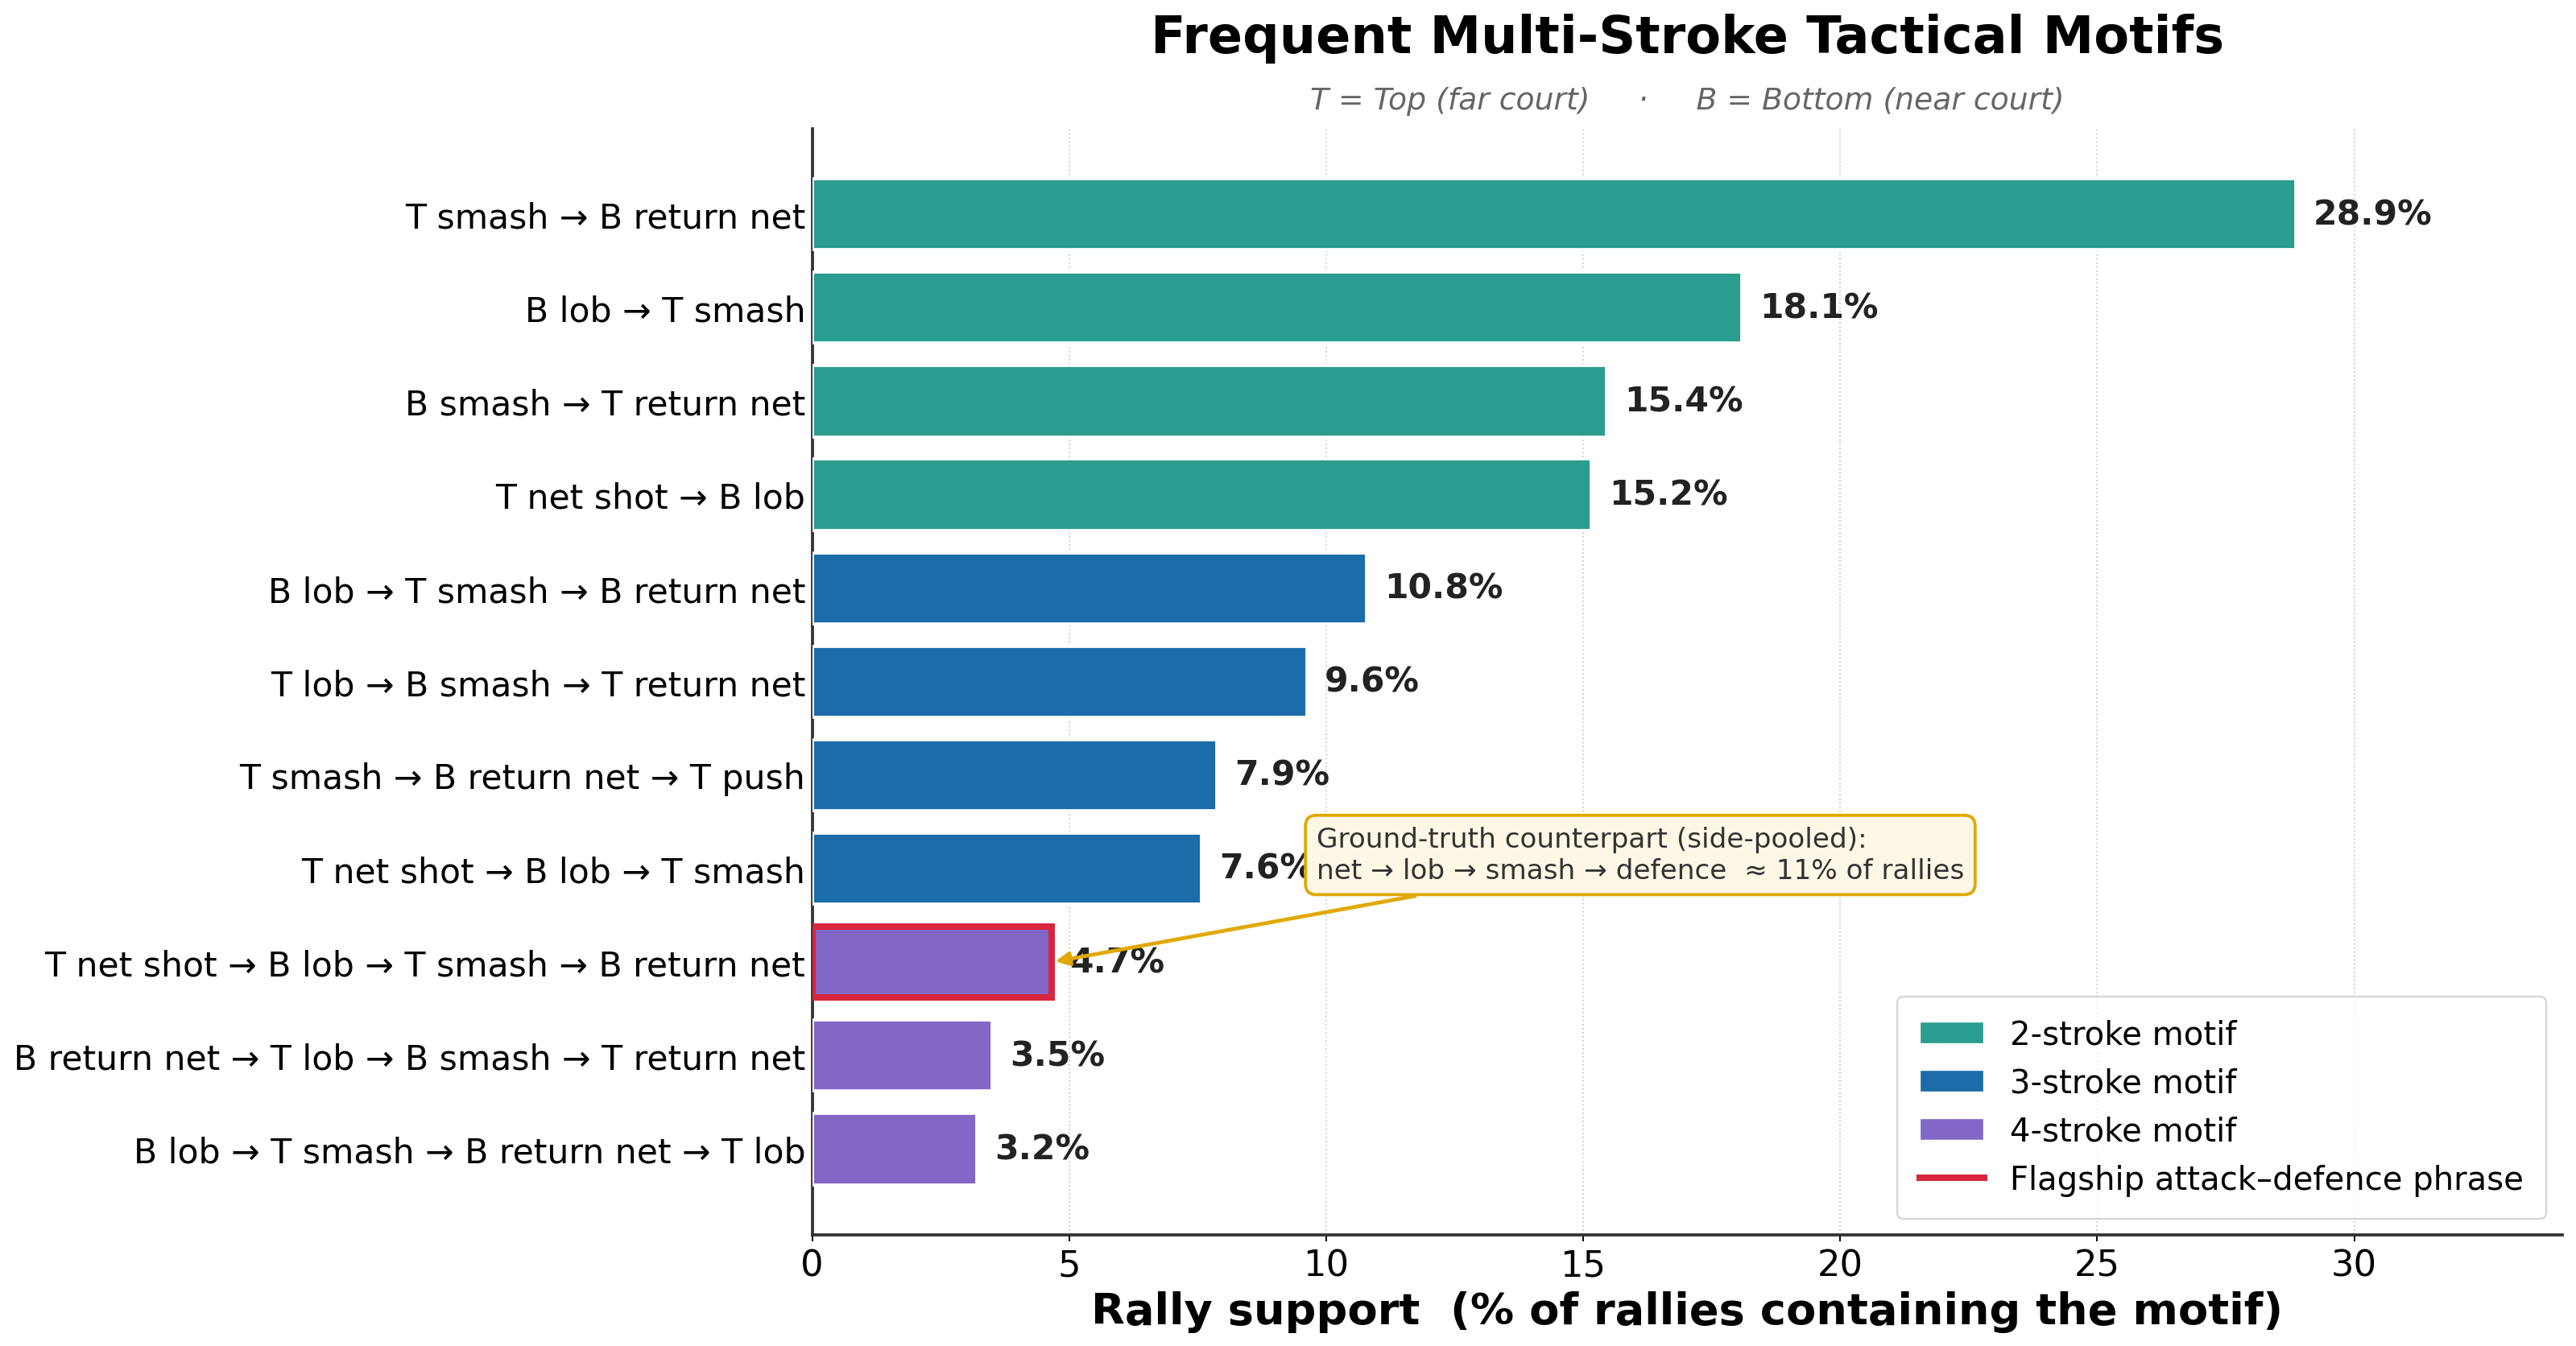
\includegraphics[width=\linewidth]{images/motif_support.png}
  \caption{\textbf{Frequent motifs.} Rally support of the most common contiguous multi-stroke motifs. Higher support indicates that the phrase appears in a larger fraction of rallies, making the repeated tactical grammar easier to interpret.}
  \label{fig:motif_support}
\end{figure}

\subsection{Movement Profiling}
Movement profiling relates spatial behaviour to stroke selection. Player
positions are projected into a player-centric normalized court frame using
ShuttleSet homographies, where $\text{forward}=1$ points toward the net and
$\text{forward}=0$ toward the baseline, so every player faces the net in the
same direction regardless of camera side. Across 2{,}300 valid events and
1{,}710 valid displacement pairs, stroke events cluster near the court centre
(Figure~\ref{fig:movement_profiling}, left), confirming the central-base
positioning expected in singles badminton.
Per-profile statistics are computed along twelve movement dimensions:
mean forward position, lateral and forward position spread, mean
inter-stroke displacement, rightward, netward, and baseline-ward displacement
rates, smash rate, net attack rate, lift/clear rate,
smash-after-large-displacement rate, and rear-court smash rate.

To quantify pairwise relationships, we compute the Pearson correlation
coefficient
\[
r = \frac{\sum_{k} (x_k - \bar{x})(y_k - \bar{y})}{\sqrt{\sum_k (x_k -
\bar{x})^2\, \sum_k (y_k - \bar{y})^2}},
\]
where $\bar{x}$ and $\bar{y}$ are sample means across profiles. Because only
$n=16$ player-set profiles enter these correlations, we report each with its
$95\%$ confidence interval and two-sided $p$-value and apply Benjamini--Hochberg
(BH) false-discovery-rate control across the full set of $\binom{12}{2}=66$
pairwise correlations from which the five below are selected; at this sample size
$|r|$ must reach roughly $0.50$ to clear raw significance. The two \emph{direct}
movement-to-attack associations do not clear it: net-ward displacement vs.\ smash
frequency is $r=+0.30$ ($95\%$ CI $[-0.23,+0.70]$, $p=0.25$) and baseline-ward
retreat vs.\ smash is $r=-0.34$ ($[-0.71,+0.19]$, $p=0.20$). Their signs match
the expected direction---forward movement preceding attack---but at $n=16$ we
treat them as \emph{suggestive, not confirmed}. The three \emph{structural}
correlations are individually significant: lateral coverage width vs.\ net-ward
frequency $r=+0.73$ ($[+0.37,+0.90]$, $p=0.001$), forward-position variability
vs.\ net-attack rate $r=+0.56$ ($[+0.09,+0.83]$, $p=0.025$), and mean forward
position vs.\ rear-court smash rate $r=-0.68$ ($[-0.88,-0.28]$, $p=0.004$). Under
the stricter full-matrix BH correction only the strongest, $r=+0.73$, retains
significance ($q=0.04$); $r=-0.68$ and $r=+0.56$ fall to $q=0.085$ and $q=0.27$,
so we report them as real but multiplicity-sensitive. The robust takeaway is
geometric---players who cover more lateral ground also press the net more
($r=+0.73$)---whereas the direct movement-to-smash link is only weakly supported
at this sample size and should be read as indicative.

\paragraph{Movement-style groups.}
Applying KMeans to the standardized 12-dimensional profiles and selecting
$k=3$ by joint silhouette and bootstrap-ARI criteria yields three distinct
movement archetypes across the 16 player-set profiles (Figure~\ref{fig:movement_clusters}).
Table~\ref{tab:movement_clusters} summarises the centroid values of the key
discriminating features.

\begin{table*}[h]
  \caption{Movement-style cluster centroids ($k=3$, silhouette 0.151, bootstrap ARI 0.365).
           Forward position: 1\,=\,net, 0\,=\,baseline. All rates are fractions.}
  \label{tab:movement_clusters}
  \centering
  \small
  \begin{tabular}{lrrr}
    \toprule
    Feature & Cluster 0 & Cluster 1 & Cluster 2 \\
            & Active Attacker & Passive Baseliner & Rear-court Dom. \\
            & ($n=8$) & ($n=3$) & ($n=5$) \\
    \midrule
    Mean forward position         & 0.482 & \textbf{0.501} & 0.379 \\
    Netward displacement rate     & \textbf{0.434} & 0.360 & 0.380 \\
    Baseline-ward displacement rate & 0.155 & 0.189 & \textbf{0.207} \\
    Smash rate                    & \textbf{0.101} & 0.064 & 0.077 \\
    Net attack rate               & 0.385 & 0.266 & \textbf{0.395} \\
    Rear-court smash rate         & 0.847 & 0.714 & \textbf{0.975} \\
    Smash after large displacement & 0.652 & 0.663 & \textbf{0.802} \\
    \bottomrule
  \end{tabular}
\end{table*}

\textbf{Cluster~0 --- Active Attacker} ($n=8$, majority): Mid-court base
($\mu_\text{fwd}=0.482$) with the highest net-ward movement rate (0.434),
the highest smash rate (10.1\%), and the highest net attack rate (38.5\%).
These player-sets actively press the net and create attacking opportunities
via overhead smashes and net pressure, representing the dominant all-round
aggressive style across the matches.

\textbf{Cluster~1 --- Passive Baseliner} ($n=3$): Despite having the most
net-forward average position ($\mu_\text{fwd}=0.501$), these profiles show
the lowest net-ward displacement rate (0.360), lowest smash rate (6.4\%), and
lowest net attack rate (26.6\%). The apparent contradiction---positioned close
to the net yet generating the fewest net attacks---suggests reactive, defensive
positioning: these players are pushed toward the net by their opponent rather
than choosing to attack it. The lowest rear-court smash rate (71.4\%) also
reflects fewer committed overhead situations.

\textbf{Cluster~2 --- Rear-court Dominator} ($n=5$): The deepest court base
($\mu_\text{fwd}=0.379$) combined with a 97.5\% rear-court smash rate tells a
coherent story: these player-sets almost exclusively smash from behind
mid-court and frequently require a large displacement to reach the shuttle
first (smash-after-large-displacement rate 80.2\%). Despite their deep base,
they also post a high net attack rate (39.5\%), pointing to full-court
coverage---retreating for overhead power, then pressing forward for net
exchanges.

\paragraph{Validation against ground truth.}
Because these archetypes are built from \emph{predicted} stroke rates, we test
how much they depend on classifier error by re-deriving the identical 16
profiles from ground-truth labels (the positional features are
label-independent, so only the five stroke-rate axes change). The predicted
stroke-rate features track their true counterparts closely across profiles, with
per-feature Pearson correlations of $0.74$--$0.84$ (mean $\bar{r}=0.79$;
Figure~\ref{fig:mining_validation}d), so the \emph{profile axes themselves are
faithful}. The discrete cluster assignment is the weaker link: the
predicted-derived and truth-derived $k{=}3$ partitions agree at an adjusted Rand
index of $0.17$ (versus $\approx0.00$ expected for random labels). This
predicted-vs-truth \emph{agreement} ARI is distinct from---and lower than---the
bootstrap \emph{stability} ARI of $0.365$ reported above, and it sits within the
noise band expected when partitioning only 16 units. We therefore present the
three movement archetypes as a descriptive summary of playing style rather than
a stable, transferable player taxonomy.

\begin{figure*}[t]
  \centering
  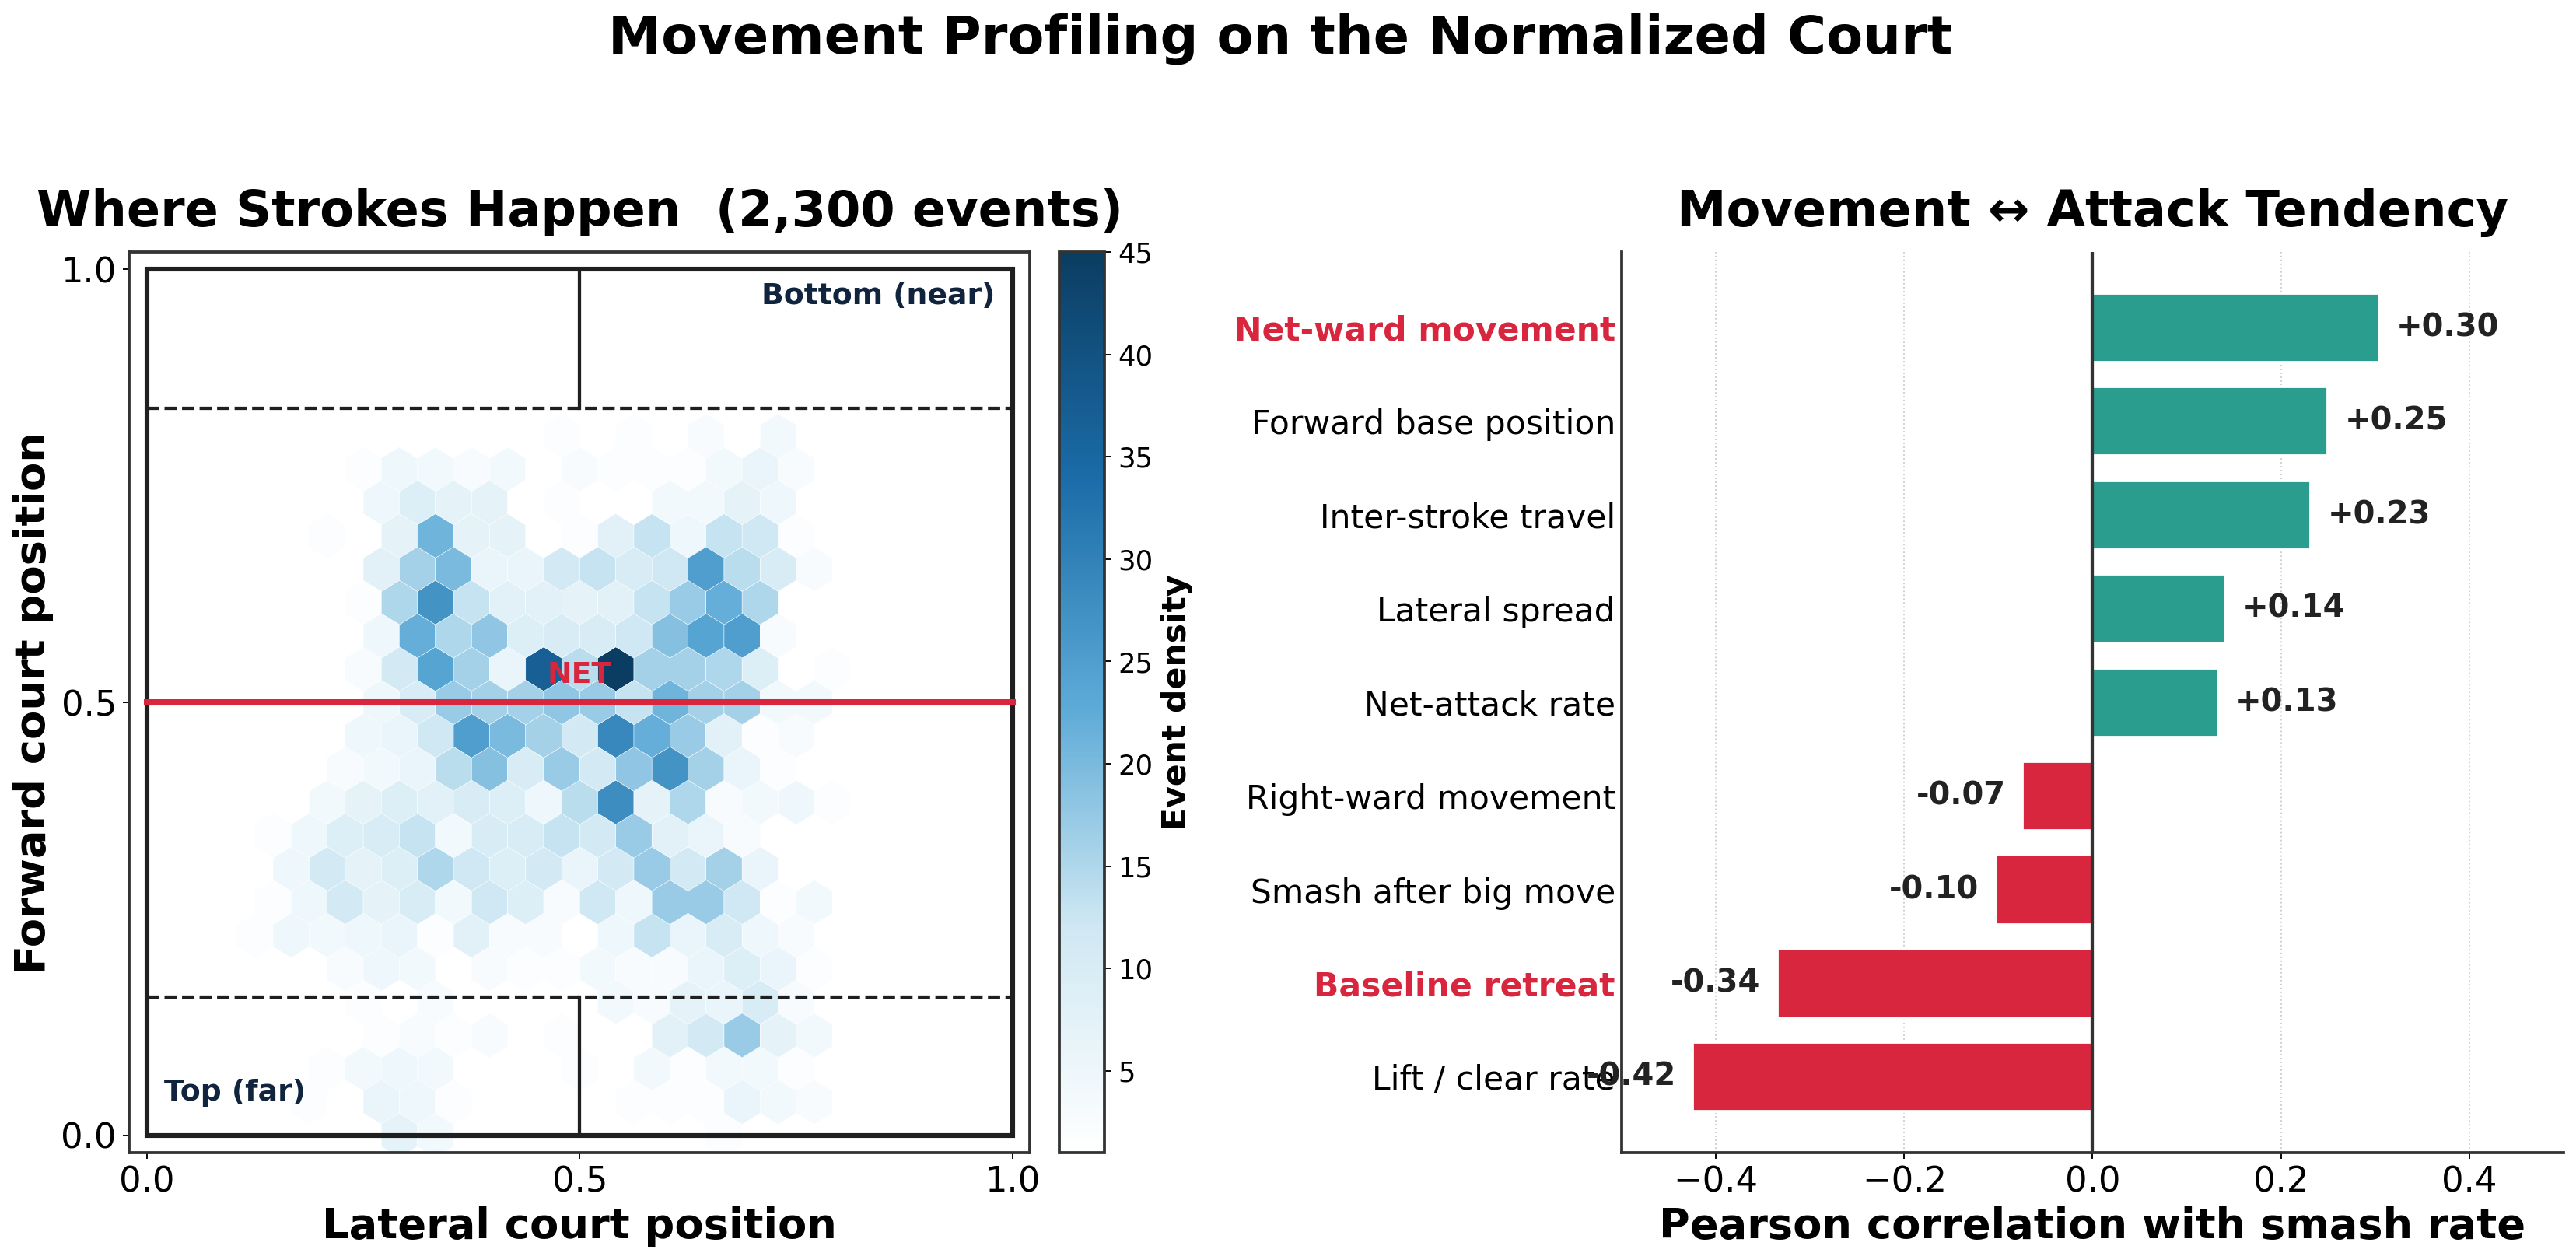
\includegraphics[width=\linewidth]{images/movement_profiling.png}
  \caption{\textbf{Movement profiling.} \emph{Left:} occupancy of 2{,}300
  stroke events on the normalized court, showing the central-base tendency.
  \emph{Right:} Pearson correlation of movement features with smash rate.
  Net-ward movement ($r=+0.30$) and baseline retreat ($r=-0.34$) point in the
  expected directions but are not significant at $n=16$ ($p>0.2$); the
  significant structural correlation is lateral coverage vs.\ net-ward frequency
  ($r=+0.73$, $p=0.001$, inter-feature, not shown here).}
  \label{fig:movement_profiling}
\end{figure*}

\begin{figure}[t]
  \centering
  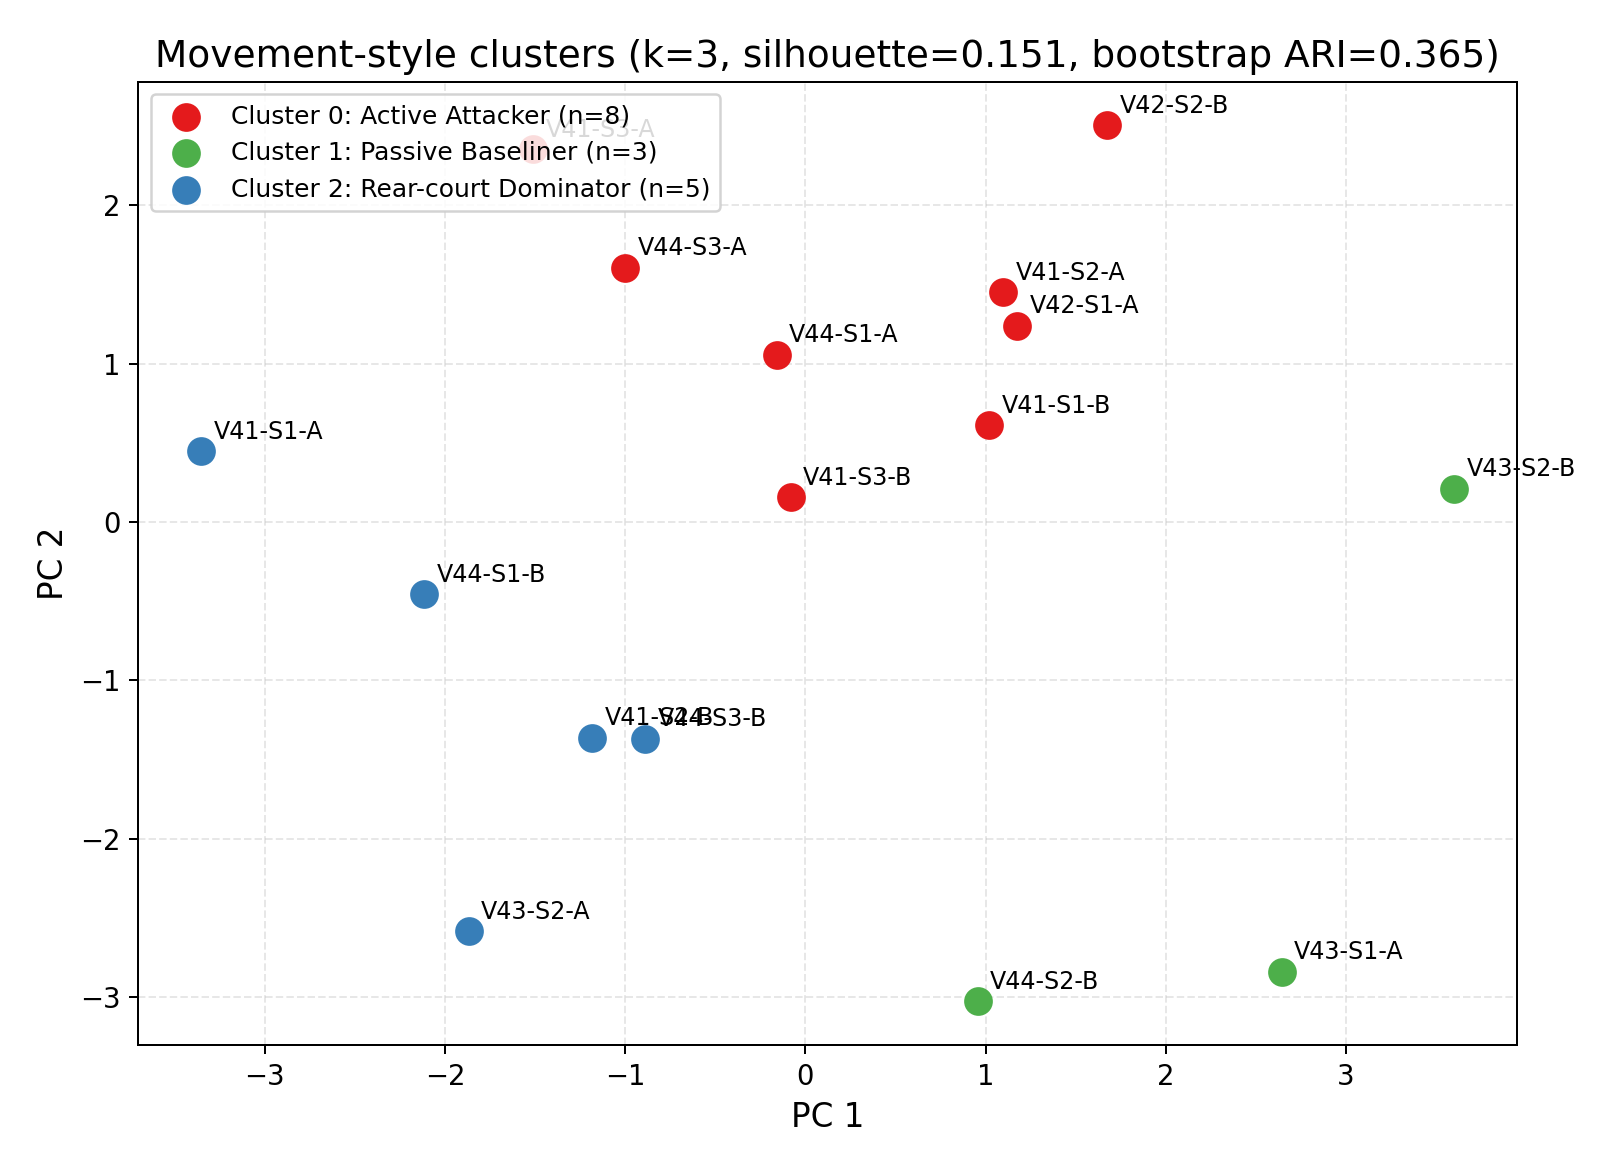
\includegraphics[width=\linewidth]{images/movement_clusters.png}
  \caption{\textbf{Movement-style clusters.} PCA projection of 16 player-set
  profiles ($k=3$, silhouette 0.151, bootstrap ARI 0.365), labelled by
  video, set, and player (A/B). \textbf{Cluster~0} (red) groups active
  attackers with the highest net-ward movement and smash rates;
  \textbf{Cluster~1} (green) groups passive baseliners with low attack rates
  despite a net-forward position; \textbf{Cluster~2} (blue) groups
  rear-court dominators who almost exclusively smash from behind mid-court
  after large displacements.}
  \label{fig:movement_clusters}
\end{figure}

\subsection{Mining Validation}

Strong perception metrics do not by themselves establish that the mined tactics
are correct: a classifier could score well per stroke yet still distort
aggregate statistics. We therefore close the loop by running each analysis on
both the predicted and the matched ground-truth labels and reporting the gap,
summarized in Table~\ref{tab:mining_eval} and visualized in
Figure~\ref{fig:mining_validation}. Four of the five views survive end-to-end
prediction well. Stroke composition stays close to truth ($\mathrm{KL}=0.04$,
$4\times$ better than uniform); the transition matrix ($\mathrm{Frobenius}=1.23$)
clearly beats both the unigram ($2.61$) and uniform-random ($2.77$) baselines,
showing that real first-order structure is recovered; and motif support rankings
correlate strongly with truth at the two- and three-stroke scale (Spearman
$0.85$ and $0.66$). The fifth view, strategy clustering, is faithful at the
feature level (mean Pearson $0.79$ between predicted- and truth-derived profiles)
but unstable at the discrete-assignment level (agreement ARI $0.17$). The overall
verdict is therefore quantitative and specific: sequence-level mining of the
predicted event stream is reliable, and the single weakest component is discrete
player clustering---not the recovered tactical grammar.

\begin{figure*}[t]
  \centering
  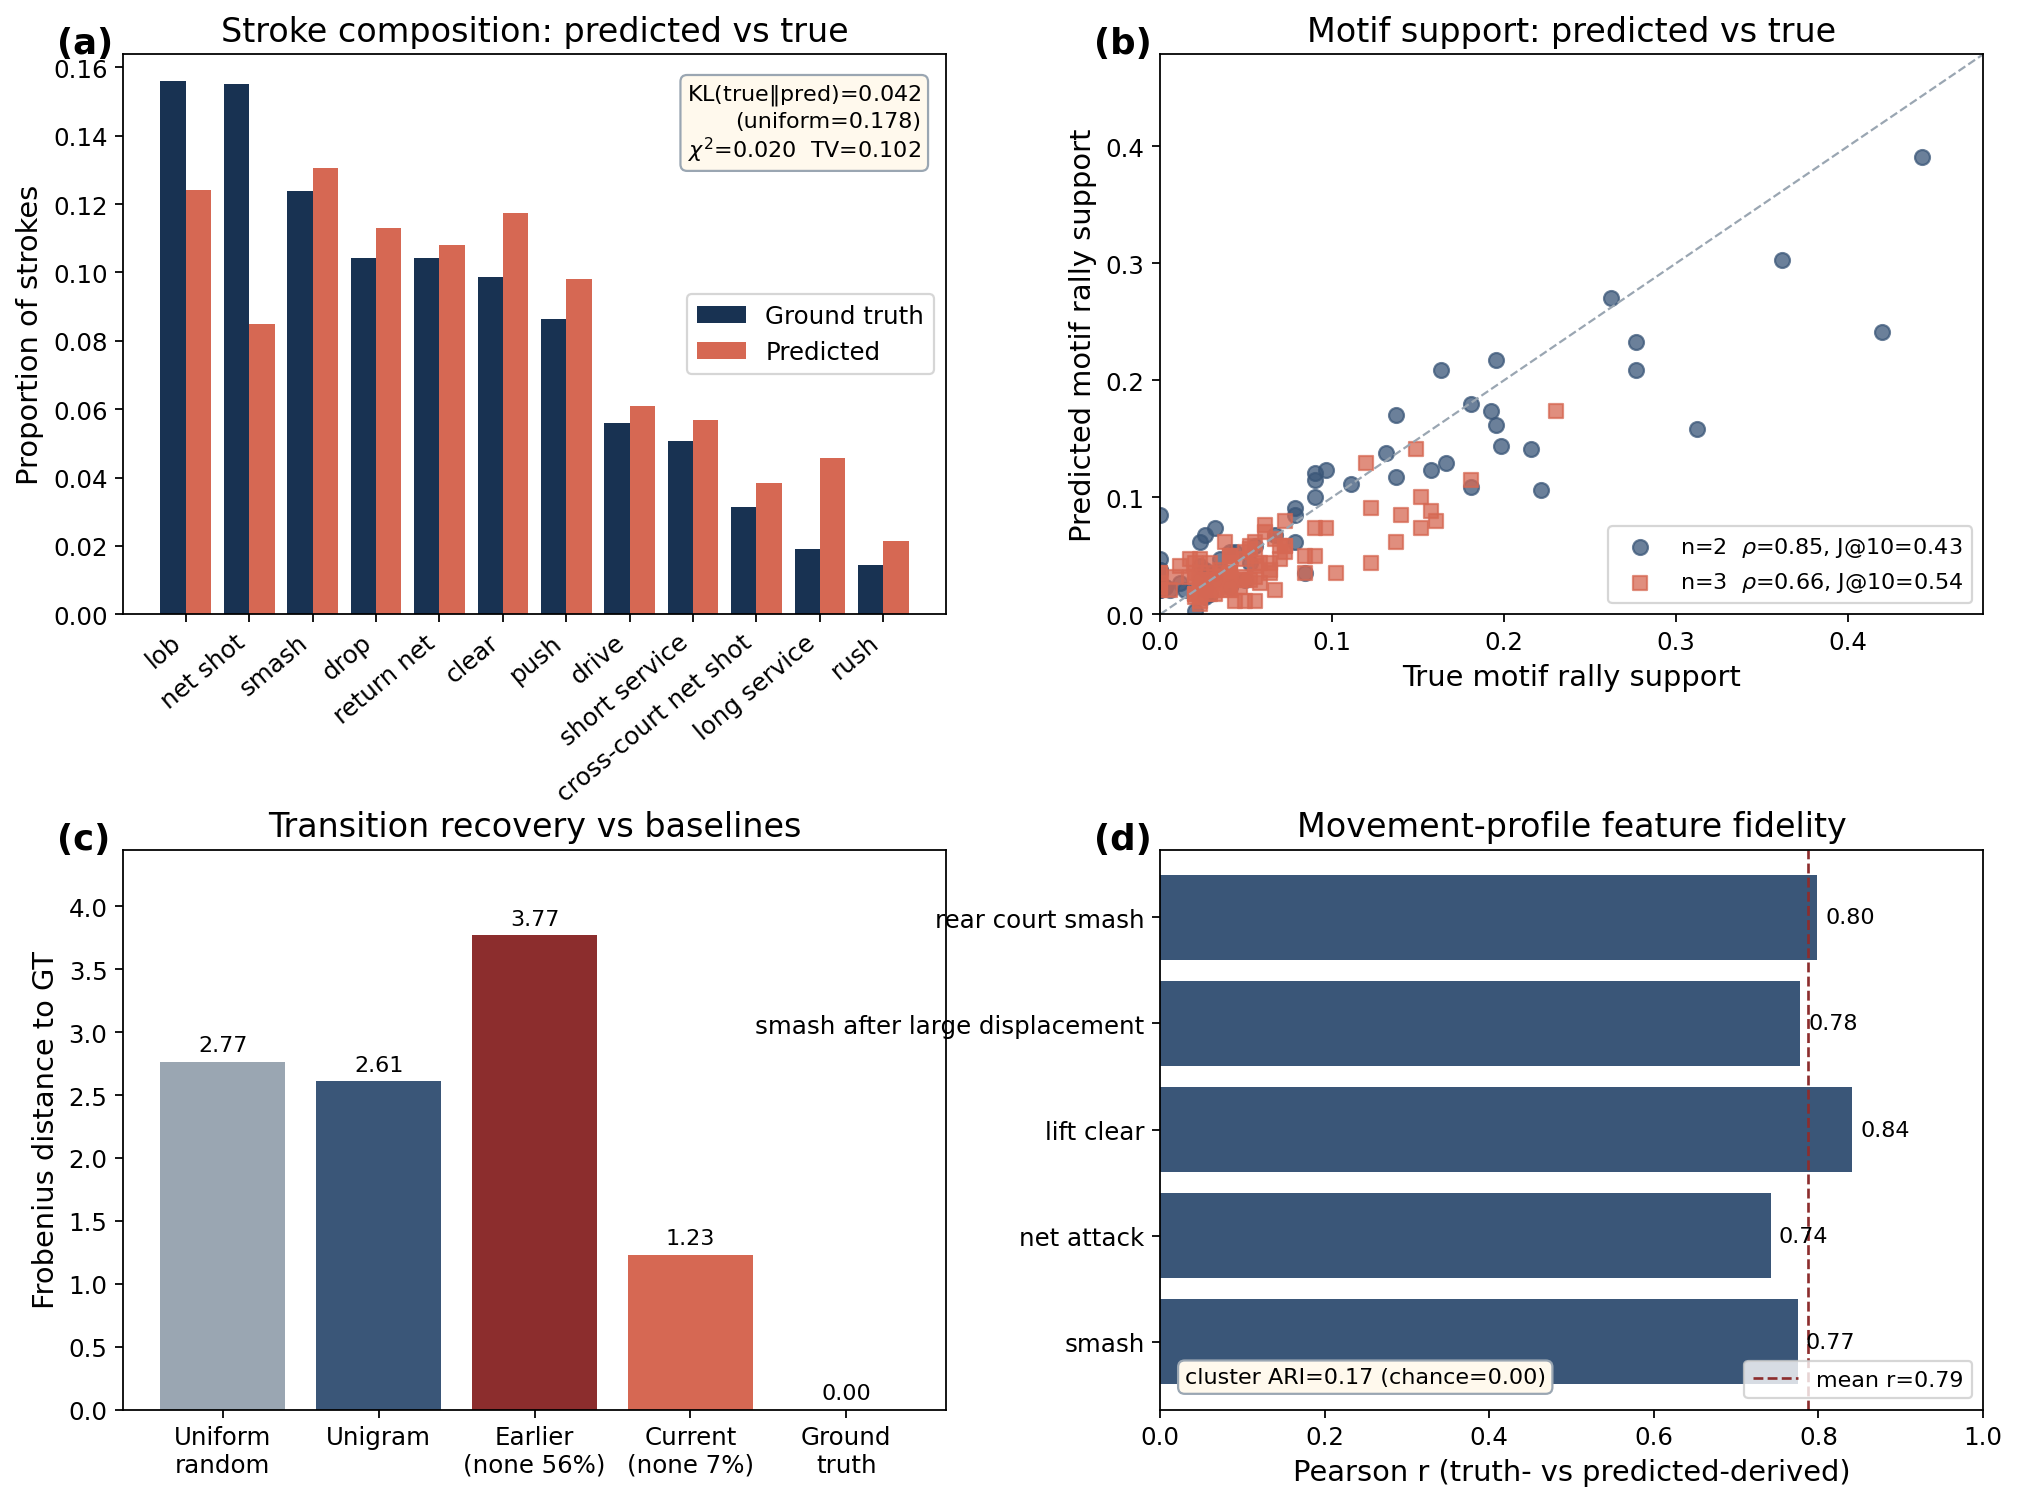
\includegraphics[width=\textwidth]{images/mining_validation.png}
  \caption{\textbf{Mining validation: predicted vs.\ ground truth on the same
  3{,}178 events.} \emph{(a)} Predicted and true stroke-type distributions stay
  close in aggregate ($\mathrm{KL}=0.04$, TV$=0.10$), though the classifier
  under-recalls net shot and lob, promoting smash to the nominal top of the
  predicted ranking. \emph{(b)} Predicted vs.\ true
  motif rally support (pairs and triples); points hug the diagonal (Spearman
  $0.85$/$0.66$), with four-gram agreement weaker ($\rho=0.32$, reported in
  text). \emph{(c)} Transition-matrix
  Frobenius distance to ground truth (all on the shared 3{,}178-event reference):
  the current pipeline ($1.23$) beats the unigram ($2.61$) and uniform-random
  ($2.77$) baselines, while the earlier \texttt{none}-flooded pipeline ($3.77$)
  is worse than chance. \emph{(d)}
  Movement-profile feature fidelity: predicted stroke-rate features correlate
  $0.74$--$0.84$ with their truth-derived values, though the discrete cluster
  agreement (ARI $0.17$) is weak.}
  \label{fig:mining_validation}
\end{figure*}